\chapter{Iterators in JavaScript} % (fold)
\label{chap:Iterators in JavaScript}
This section explains the concept of iterable and iterator objects and points
out features and characteristics of it. |Sequence| is one implementation of
an iterable and represents the core functionality of the implementations
related to the functional standard library. We call these functionalities in
the thesis Sequence library analogous to the package in the code
base~\cite{wildwyss_kolibri}. The following
discussion covers challenges and solutions for creating a robust and
user-friendly API.

\section{Iterables in General}
\label{sec:Iterables in General}
In Computer Science, iterators are a popular concept. An iterator provides
access to elements of a data structure. It does not matter if the iterator
accesses a data structure fully kept in memory (like arrays) or if it computes
the elements lazily when queried. In both ways, a function call on the iterator
retrieves the next value. Iterators are an essential part of this work.
Therefore, it is crucial to understand the fundamentals of this concept. The
following sections cover this topic in depth.

\subsection{Iterable Data Structures in JavaScript}
\label{sub:Iterable data structures in JS}
JavaScript knows two protocols which define how an object can be used for
iteration. An iterable object, also known as an iterable, represents a
collection of data. By calling a function on the iterator, we can access the
next element in the collection, moving in a single direction. Iterators can be
either finite or infinite. Once a finite iterator reaches its end, it is
considered "used up" - subsequent calls to such an exhausted iterator won't
produce any meaningful results. Below, we will provide a more detailed
description of these two protocols.

\subsubsection{The Iterable Protocol}
\label{subsub:The Iterable Protocol}

In JavaScript, an object is considered an iterable if it contains a property
called |[Symbol.iterator]|. This property signifies that the object is of type
|Iterable<T>|. When we invoke the |[Symbol.iterator]| property, it creates an
iterator that follows the iterator protocol explained in the following section.
Objects in JavaScript that implement this property can be utilized with
destructuring \footnote{The destructuring assignment syntax is a JavaScript
expression that allows to extract items of iterables into individual
variables.}and |for...of| loops. Listing \ref{lst:iterable_protocols}
showcases an example of an object defining the |[Symbol.iterator]| property.

\begin{lstlisting}[
  style=ES6, 
  caption=Iterable protocol,
  label={lst:iterable_protocols}
  ]
  return {
    [Symbol.iterator]: () => {
      return { next: next }; *'// next is defined in~\ref{lst:iterator_protocol}'*
    }
  }
\end{lstlisting}

\subsubsection{The Iterator Protocol}
\label{subsub:The Iterator Protocol}
Invoking the |[Symbol.iterator]| property obtains an iterator object
complying to the iterator protocol. It must implement a function |next|, which
defines how and which values are returned when iterating. Each iteration on an
iterator calls this function. |next| returns an object, which must
include two properties: |value| and |done|. The property |value|
contains the current value of the iteration, while |done| represents the
information on whether the end of the iteration has been reached. The following
code \ref{lst:iterator_protocol} shows a simple implementation of it. Each call
on |next| returns an object with the |value 1|. |done| is always |false|, so
the iteration never ends. 

\begin{lstlisting}[
  style=ES6, caption=Iterator protocol,
  label={lst:iterator_protocol}
  ]
  const next = () => {
    return { done: false, value: 1 };
  };
\end{lstlisting}

\subsubsection{Creating Iterables}
\label{subsub:Creating Iterables}
By combining these two protocols, the result could look like listing
\ref{lst:protocols}. The constructor |InfiniteOnesIterable| on
line~\ref{line:ctor_infiniteones} wraps the two
previously defined implementations. This constructor therefore returns iterable
objects. Since the return value is always one(|1|), this is an iterable of
type |Iterable<Number>|.

\begin{lstlisting}[
  style=ES6, caption=Iterable and iterator protocol,
  label={lst:protocols}
  ]
 const InfiniteOnesIterable = () => {*'\label{line:ctor_infiniteones}'*

  const next = () => {
    return { done: false, value: 1 };
  };

  return {
    [Symbol.iterator]: () => {
      return { next: next };
    }
  }
};

const [one, anotherOne, andOneAgain] = InfiniteOnesIterable();*'\label{line:infiniteones_destructuring}'*

for(one in InfiniteOnesIterable){
  ...
  break;
}*'\label{line:infiniteones_forof}'*


\end{lstlisting}

Because |InfiniteOnesIterable| adheres to the JS iteration protocols, it is now 
possible to create iterable objects. Language features like |for..of| and 
destructuring can process these objects as shown on line~\ref{line:infiniteones_destructuring}
to~\ref{line:infiniteones_forof}. However, beware of this 
case. This would lead to an infinite loop because the property |done| never 
becomes |true|. Therefore, the iteration never ends. We will see examples 
with non-endless iterables later in this work. 
For now, the focus here is on the protocols. Therefore, this 
example is sufficient at this point.
\newline
Such protocols make it possible to build customized iterables and
collections. This opens new possibilities. Various programming tasks can have 
different, more straightforward solving approaches in a more declarative way to
write.
There are already some JavaScript iterables present. Arrays and
|HTMLCollection|s are probably the most prominent of these.

\subsection{Types of Iterables}
\label{sub:Types of Iterables}
Previously we saw a distinction between iterables and iterators. These abstractions
also have their types. Listing \ref{lst:iterable_types} shows an excerpt of the
relevant types.

\begin{lstlisting}[
  style=ES6, caption=Types of iterables,
  label={lst:iterable_types}
  ]
// lib.es2015.iterable.d.ts

interface Iterable<T> {*'\label{line:start_iteration_types}'*
    [Symbol.iterator](): Iterator<T>;
}

interface Iterator<T, TReturn = any, TNext = undefined> {
  next(...args: [] | [TNext]): IteratorResult<T, TReturn>;
    return?(value?: TReturn): IteratorResult<T, TReturn>;
    throw?(e?: any): IteratorResult<T, TReturn>;
}*'\label{line:end_iteration_types}'*

type IteratorResult<T, TReturn = any> = IteratorYieldResult<T> *'\label{line:start_iteration_result_types}'*
                                      | IteratorReturnResult<TReturn>;


interface IteratorYieldResult<TYield> {
    done?: false;
    value: TYield;
}

interface IteratorReturnResult<TReturn> {
    done: true;*'\label{line:iteration_return_result_done}'*
    value: TReturn;
} *'\label{line:end_iteration_result_types}'*
\end{lstlisting}

\begin{itemize}
  \item{Line~\ref{line:start_iteration_types}~-~\ref{line:end_iteration_types}: 
      An |Iterable| is of type |Iterable<T>|, whereas the object returned by the property
      |[Symbol.Iterator]| is of type |Iterator<...>|. An |Iterator| requires having a property |next|. 
      This is the function that returns values when iterating. These values must be 
      of type |IteratorResult<...>.|
    }
  \item{Line~\ref{line:start_iteration_result_types}~-~\ref{line:end_iteration_result_types}:
      |IteratorResult<...>| itself is defined to return an 
      object of type |IteratorReturnResult<...>|, which either is of type
      |IteratorYieldResult| or |IteratorReturnResult|. This object contains the actual 
      values we want to work with.}
\end{itemize}

In chapter~\ref{subsub:Stateful Decorating}, we will see the reason for this
nested architecture of the JS iteration protocol.

\subsubsection{Closer Look to IteratorReturnResult}
\label{subsub:Closer look to IteratorReturnResult}
When iterating an iterable, the returned elements are of type
|IteratorYieldResult<T>|. The last and all following element of an iterable is of type
|IteratorReturnResult<TReturn>|. This ensures that |done| is set to |true|, as 
can be seen on line~\ref{line:iteration_return_result_done} in listing~\ref{lst:iterable_types}.

\subsection{Illustration of the JS Iteration Protocol}
\label{sub:Illustration of the JS Iteration Protocol}
Listing~\ref{lst:example_js_iteration_protocol} illustrates the behavior of the
JS iteration protocol more clearly using a sample scenario. Since array is an
iterable, we can use it for the following demonstration:

\begin{lstlisting}[
  style=ES6, 
  caption=Example: JS Iteration Protocol,
  label={lst:example_js_iteration_protocol}
  ]
// array including two values, 0 and 1
const list = [0, 1];
const iterator = list[Symbol.iterator]();*'\label{line:illustraion_create_iterator}'*

iterator.next(); // returns { done: false, value: 0 }
iterator.next(); // returns { done: false, value: 1 }
iterator.next(); // returns { done: true,  value: undefined }
iterator.next(); // returns { done: true,  value: undefined }
\end{lstlisting}

On line~\ref{line:illustraion_create_iterator}, invoking |[Symbol.iterator]|
returns iterator of the iterable |list|. 
After that, we call |next| four times directly on the iterator. Since the
iterable contains only two elements, the third and fourth call on |next|
returns an object of type |IteratorReturnResult<TReturn>|. Thereby, |done| is
|true| and |value| is |undefined|. \\
By using |for...of| and destructuring, an iterable would stop iterating at this
point. This means an |for...of| loop runs until the property |done| is set to
|true|.

\section{Sequence: An iterable Series of Values}
\label{sec:Sequence: A Series of Values}
In Computer Science, naming elements accurately poses a significant challenge 
when aiming to develop sustainable and robust code. We decided to name series
of data a "sequence". It has been influenced by several factors:

\begin{itemize}
  \item Sequences are not conventional lists known from other programming
    languages.
\item The name sequence is already known from mathematics.
\item Giving this data structure a more familiar name, for example "list",
  leads to wrong assumptions. 
\end{itemize}
What distinguishes the object generated by the sequence from the conventional
list is that a sequence generates its values when they are requested.
Therefore, it needs almost no memory. At the same time, you have the impression
that you are dealing with a vast amount of data. So the constructor |Sequence|
emerged, which generates such connected data.

\subsection{Components of a Sequence}
\label{sub:Components of a Sequence}
Defining a sequence requires specifying three essential points:
\begin{enumerate}
  \item{A fixed starting value for the sequence} 
  \item{A function that determines whether the sequence should generate
    further values} 
  \item{A function to calculate the next value based on its predecessor} 
\end{enumerate}
These three elements define the sequence. Listing \ref{lst:sequence} on
line~\ref{line:seq_args} shows the passing of these three elements as arguments
to the constructor. To keep the focus on the core elements of the sequence,
some functionality in listing \ref{lst:sequence} is omitted and discussed later.
The |next| function, explained section~\ref{subsub:The Iterator Protocol}, is on
lines~\ref{line:start_protocol}~-~\ref{line:end_protocol}. It contains the
logic to return the next value in an iteration. First, it uses |whileFunction|
to check if the Sequence has finished. If this is not the case, the
|incrementFunction| calculates the next element, which afterward will be
returned.

\begin{lstlisting}[
  style=ES6, 
  caption=Parts of Sequence,
  label={lst:sequence}
  ]
// Sequence.js
const Sequence = (start, whileFunction, incrementFunction) => {*'\label{line:seq_args}'*

  const iterator = () => {
    let value = start;
    /**
     * @template _T_
     * Returns the next iteration of this iterable object.
     * @returns { IteratorResult<_T_, _T_> }
     */
    const next = () => {*'\label{line:start_protocol}'*
      const current = value;
      const done = !whileFunction(current);
      if (!done) value = incrementFunction(value);
      return { done, value: current };*'\label{line:end_protocol}'*
    };

    return { next };
  };

  return ... 
};
\end{lstlisting}

\subsection{Using a Sequence}
\label{sub:Using a Sequence}
Listing \ref{lst:even-sequence} shows the definition of a sequence of even 
numbers smaller than ten and how to use it. 
\begin{lstlisting}[
  style=ES6, 
  caption=Sequence of even numbers,
  label={lst:even-sequence}
  ]
const startValue        = 0;
const whileFunction     = x => x < 10;
const incrementFunction = x => x + 2;

const seq = Sequence(startValue, whileFunction, incrementFunction);

for (const elem of seq) {
  console.log(elem);
}
// => Logs '0, 2, 4, 6, 8' *'\label{line:demo_output}'*
\end{lstlisting}

The |for..of| loop iterates over the sequence until |done| is true. Meanwhile,
|console.log| writes the elements to the console.
Line~\ref{line:demo_output} shows the output produced.


\subsection{Range - A Real-World Example}
\label{sub:Range - A Real-World Example}
When considering sequences, a common requirement is to generate a series of
numbers, often with a specified starting point, an end value, and adjustable
increments. This is a classic definition of implementing a Range.
Ranges are built into many programming languages such as
Haskell~\cite{haskell_list},
Python~\cite{python_range}
or Kotlin~\cite{kotlin_ranges}. Therefore, we also implemented a Range using the Sequence constructor. 

Listing~\ref{lst:range_haskell} shows the construction of a Range in Haskell.
\begin{lstlisting}[
  style=Haskell,
  caption=Range in Haskell,
  label={lst:range_haskell}
]
ghci> r = [1..10] -- contains the numbers from 1 up to 10.
ghci> r
[1,2,3,4,5,6,7,8,9,10]
ghci> r = [1..] -- contains an infinite range
\end{lstlisting}

Listing~\ref{lst:kolibri_range} demonstrates different ways to initialize a
Range of the Sequence library.

\begin{lstlisting}[
  style=ES6, 
  caption=Kolibri toolkit Range,
  label={lst:kolibri_range}
  ]
 const range               = Range(3);
 const [five, three, one]  = Range(1, 5, -2);
 const [three, four, five] = Range(5, 3);
\end{lstlisting}

\subsubsection{What can a Range be used for?}
\label{subsub:What can a Range be used for?}
Ranges offer efficient processing of sequences of almost any size, consuming
minimal memory and computational resources. As a result, they serve as
excellent foundational components for larger structures. Due to their ability
to handle number sequences, ranges have versatile applications. They can be
utilized for lazily generating numbers or executing a specific action several
times.

\subsubsection{The Boundaries}
\label{subsub:The Boundaries}
Built-in ranges are commonly available in various programming languages, making
their usage in the Kolibri toolkit intuitive. However, it is important to note
that not all languages handle range boundaries similarly. For instance, Kotlin
and Haskell consider both boundaries inclusive. Thus, a range from 1 to 3 in
these languages would include the elements 1, 2, and 3. On the other hand, in
Python, only the lower limit is inclusive. Therefore, the boundaries must be
set as 1 and 4 to create an equivalent range in Python.
Since it seems more intuitive to have both borders inclusive, the range for
Kolibri toolkit works accordingly.

\subsubsection{Implementation}
\label{subsub:Implementation}
A Range uses a Sequence under the hood. Helper functions analyze the parameters
and, if necessary, reorder them to return a desired Sequence. Listing~\ref{lst:impl_range} shows the
main part of the implementation of the Range. 

\begin{lstlisting}[
  style=ES6, 
  caption=Implementation of the Range,
  label={lst:impl_range}
  ]
/**
 * @constructor
 * @pure
 * @param { !Number } firstBoundary  - the first boundary of the range
 * @param { Number }  secondBoundary - optional second boundary of the Range
 * @param { Number }  step - size of a step, processed during each iteration
 * @returns SequenceType<Number>
 */
const Range = (fstBoundary, sndBoundary = 0, step = 1) => {
  const stepIsNegative = 0 > step;
  const [left, right] = normalize(fstBoundary, sndBoundary, stepIsNegative);

  return Sequence(
    left,                                                // start value
    value => hasReachedEnd(stepIsNegative, value, right),// while function
    value => value + step                                // increment function
    );
};
\end{lstlisting}

In the following, we have a closer look at the features of a Range. By doing
so, we cover the functions |normalize| and |hasReachedEnd| to explain them 
in more detail.

\subsubsection{Features}
\label{subsub:Features}

\begin{itemize}
  \item{\textbf{Parametrization:} The range can be initialized with 1-3 parameters. The parameters specify the lower limit, the upper limit and the
  step size. If not all parameters are set the range uses suitable default values.}
  \item{\textbf{Interchangeable boundaries:} Interchangeable lower and upper limits when creating a new range}
  \item{\textbf{Negative boundaries and step:} The boundaries and the step size of the range can be positive or negative integers.}
\end{itemize}

\subsubsection{Normalization of the Boundaries}
\label{subsub:Normalization of the Boundaries}
To ensure flexibility, the Range provides the interchangeability of boundaries
and the option for positive or negative step values. Initially, the range
boundaries are normalized based on the step value. This normalization
determines which boundary will contain the first generated number and which
will represent the last number.
The following figure~\ref{fig:norm-flowchart} explains the process in detail.

\begin{figure}[H]
    \centering
    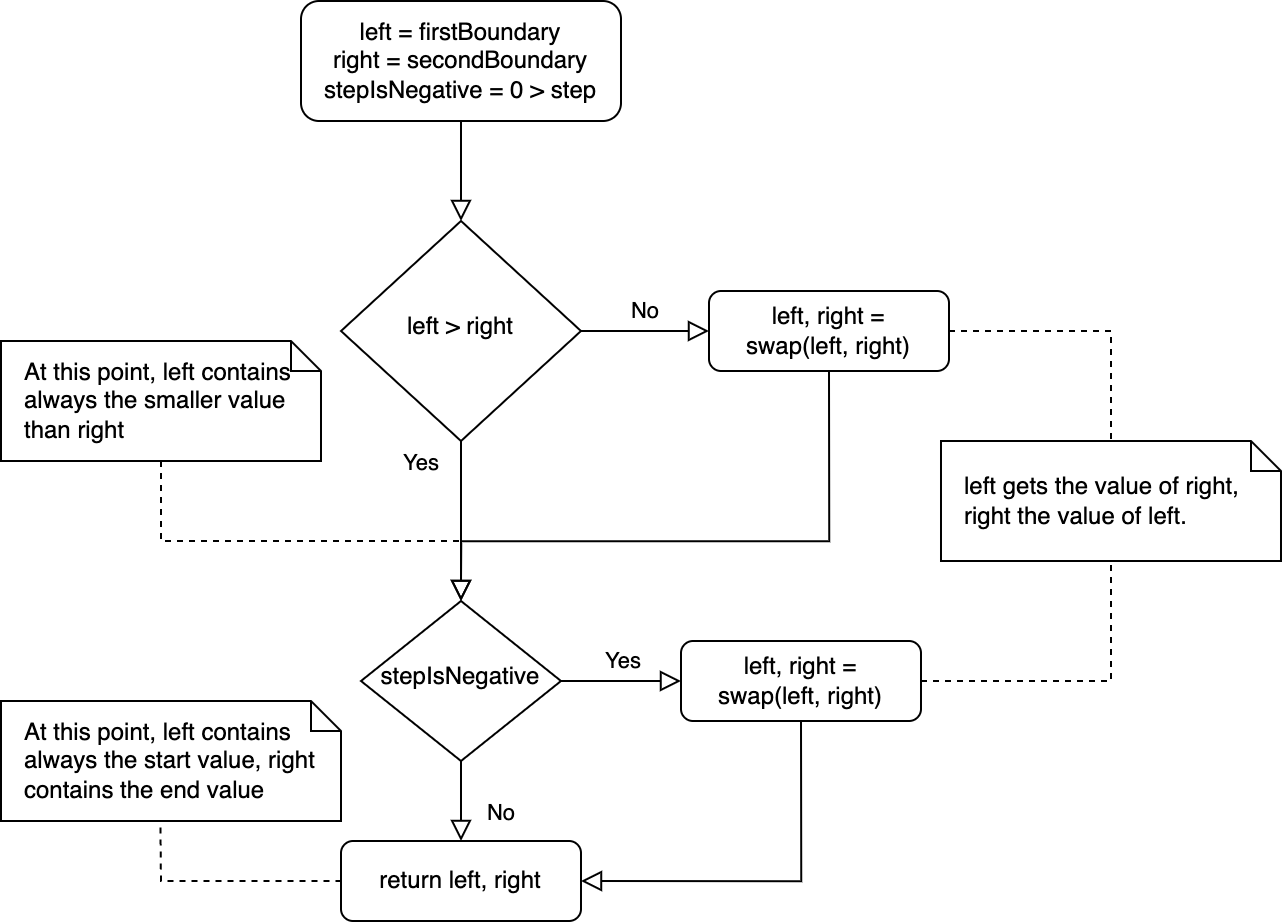
\includegraphics[width=0.9\textwidth]{mainmatter/pictures/boundary-normalization.png}
    \caption{Normalization Flow-Chart diagram}
    \label{fig:norm-flowchart}
\end{figure}

\subsubsection{The End of a Range}
\label{subsub:The End of a Range}
The |hasReachedEnd| function detects the end of the Range and defines the
|untilFunction| of the underlying Sequence. Listing~\ref{lst:impl_hasReachedEnd}
shows the implementation of the function. 

\begin{lstlisting}[
  style=ES6, 
  caption=hasReachedEnd implementation,
  label={lst:impl_hasReachedEnd}
  ]
/**
 * Determines if the end of the range is reached.
 * @param   { Boolean } stepIsNegative
 * @param   { Number }  next - the current element of the Range
 * @param   { Number }  end  - max value of the Range
 * @returns { boolean }
 */
const hasReachedEnd = (stepIsNegative, next, end) =>
    stepIsNegative ? next >= end : next <= end;
\end{lstlisting}

The function must be able to distinguish between two different cases:

\begin{itemize}
  \item{If the step size is a negative, the Range counts from top to bottom:
    The Range reached its end as soon as next is greater or equals than right.}
  \item{If the step size is positive, the Range counts from bottom to top: The
  Range reached its end as soon as next is smaller or equals than the value right.}
\end{itemize}

\subsubsection{Some Restrictions of Using a Range}
\label{subsub:Some Restrictions of Using a Range}
We defined some Range behaviors by contract rather than intercepting or
addressing them in implementation. Therefore, we defined the following
restrictions:

\begin{itemize}
  \item{End value may not be reached exactly, but will never be exceeded.}
  \item{Zero step size leads to infinite loops, returning always the same values.}
  \item{Only values that behave correctly with respect to addition and size
    comparison may be passed as arguments.}
\end{itemize}


\subsubsection{Using a Range}
\label{subsub:Using a Range}
Following listing~\ref{lst:range_examples} demonstrates various ways to
construct a Range.

\begin{lstlisting}[
  style=ES6, 
  caption=Range examples,
  label={lst:range_examples}
  ]
// typical cases
for (const value of Range(3)) { console.log(value); }
// => Logs '0, 1, 2, 3'

for (const value of Range(2,3)) { console.log(value); }
// => Logs '2, 3'

// lower and upper boundaries interchanged
for (const value of Range(3,2,1)) { console.log(value); }
// => Logs '2, 3'

// negative step size
for (const value of Range(4,6,-2)) { console.log(value); }
// => Logs '6, 4'

for (const value of Range(6,4,-2)) { console.log(value); }
// => Logs '6, 4'

// range with negatgive boundary
for (const value of Range(0,-2,-1)) { console.log(value); }
// => Logs '0, -1, -1'
\end{lstlisting}

\subsection{Conclusion}
\label{sub:iterable_protocol_Conclusion}
Now, we discussed the ability to generate arbitrary sequences of data. However, 
just creation is often not enough as there is a need to manipulate the data or 
introduce additional levels of abstraction. In the upcoming chapter, we will 
delve into processing such Sequences.

% chapter Iterators in JavaScript (end)
